% !TEX root = ../main.tex
\section{Priority scenarios}
\label{sec:priority}

Table~\ref{tab:storms} summarises the four backtest typhoons on their observed tracks: ferry routes cancelled, people cut off on the network, mean $A$ and $R$ over the \nUnits{} units, the number of provinces in the two action tiers, and the province ranked first.

\begin{table}[htbp]
\centering
\caption{The four backtest typhoons, observed tracks (local name, with the international name and season).}
\label{tab:storms}
\footnotesize
\begin{tabularx}{\linewidth}{@{}L r r r r c L@{}}
\toprule
typhoon & ferry routes cut & people cut off & mean $A$ & mean $R$ & deploy / pre-position & top priority \\
\midrule
\tablerows{storms}
\bottomrule
\end{tabularx}
\end{table}

\subsection{Ompong 2018}

Ompong made landfall in Cagayan on \landfallOmpong{}. The model, trained on data to the landfall week only, puts \textbf{\topOmpong{}} first, with \deployOmpong{} provinces in the \enquote{deploy mobile clinics} tier and \preposOmpong{} in \enquote{pre-position supplies} (Figure~\ref{fig:priority}). \enquote{Deploy} needs at least \tierDeployA{} of people cut off. Of the four observed tracks, with observed flood, \nStormsDeploy{} put any province there; the hazard-proxy shifted tracks of Ompong put \proxyDeployOmpong{} provinces there. Figure~\ref{fig:scatter} places every unit on the risk and access axes with the provisional tier thresholds.

The dashboard repeats this for every storm and \nShifted{} shifted variants of each track ($\pm$\shiftLat\textdegree{} north or south, $\pm$\shiftLon\textdegree{} east or west), so a health officer can ask \enquote{what if it comes in further south?} and get an answer in seconds.

\begin{figure}[htbp]
\centering
\begin{minipage}[t]{0.47\linewidth}
\centering
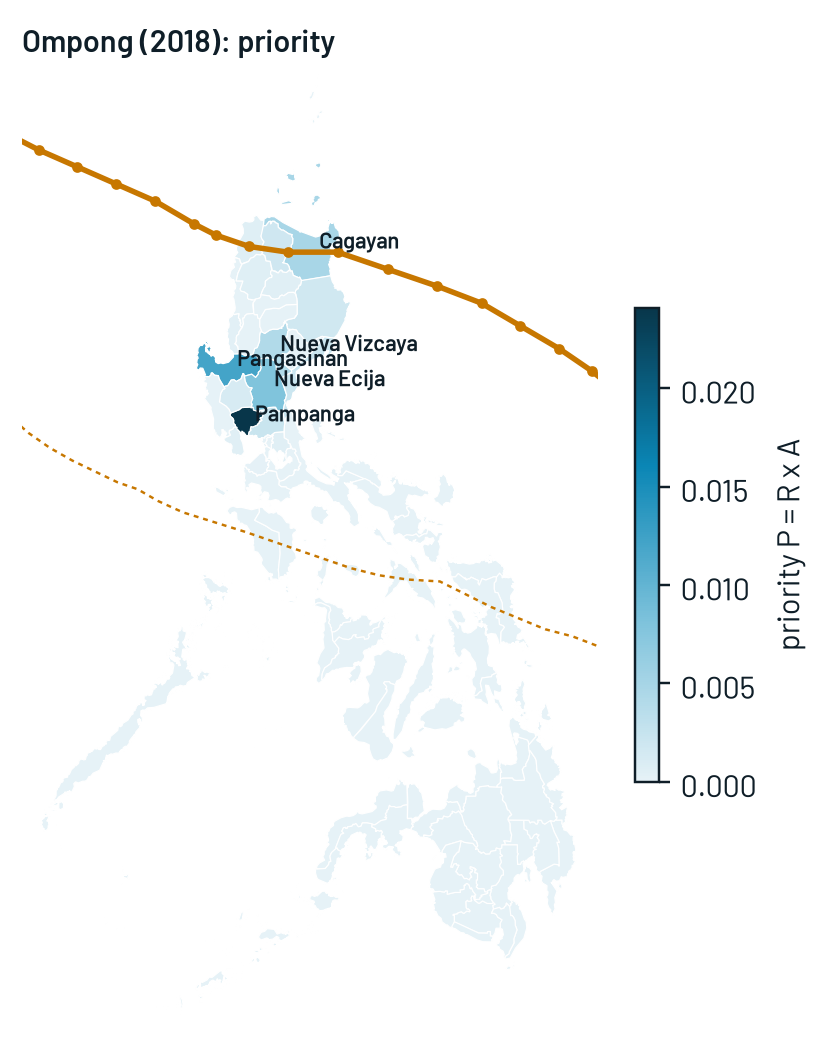
\includegraphics[width=\linewidth]{f07_priority_ompong}
\caption{$P = R \times A$ for Ompong with its track and gale swath; the top five are labelled.}
\label{fig:priority}
\end{minipage}\hfill
\begin{minipage}[t]{0.5\linewidth}
\centering
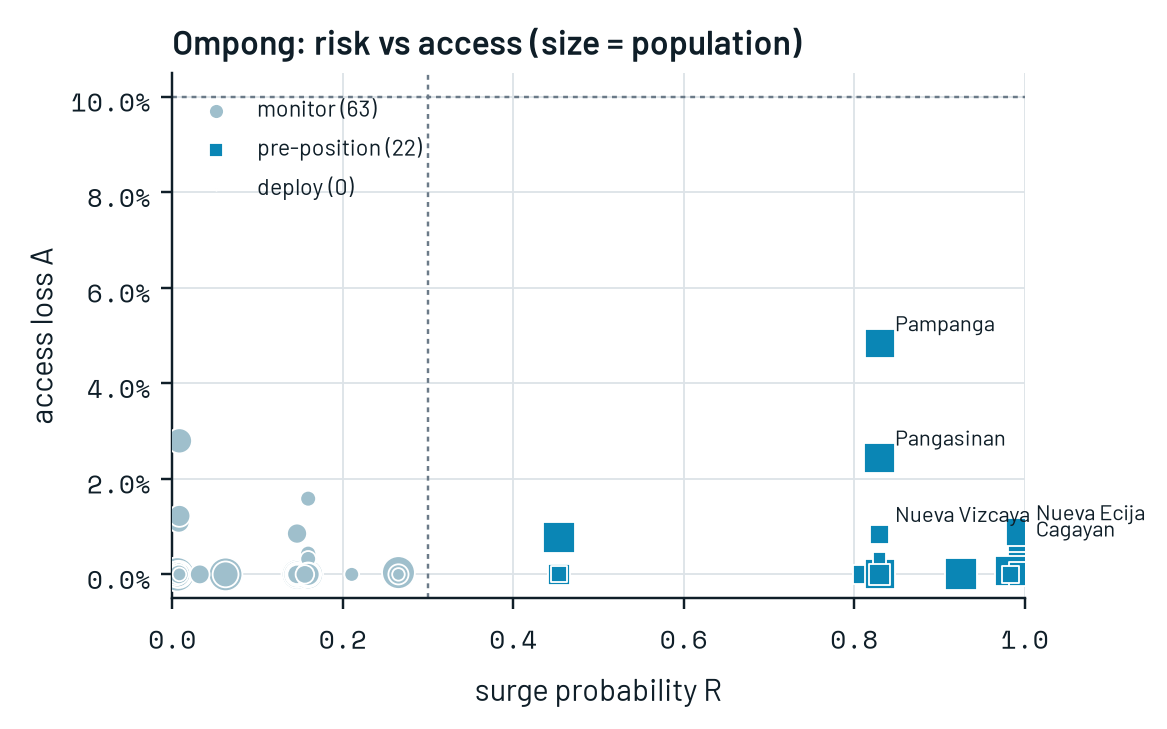
\includegraphics[width=\linewidth]{f09_scatter}
\caption{Risk against access for Ompong. Dotted lines are the provisional tier thresholds ($R = \tierPreR$, $A = \tierDeployA$); marker shape gives the tier.}
\label{fig:scatter}
\end{minipage}
\end{figure}

\subsection{Every storm, \catYearMin--\catYearMax}
\label{sec:catalog}

Beyond the four backtests, the build scores the observed track of every other storm whose gale swath touched Philippine land: \textbf{\nCat{} storms}. Each uses the latest model fitted before its week (never later data), $R$ calibrated where enough past outcomes exist (\nCalCat{} of \nCat{}), and \textbf{the NOAH 25-year proxy for flood}, since no radar map exists for them, so their cut-off counts are upper bounds. \nSkipped{} storms of 2016 are skipped: their model would have under \minHistory{} weeks of history. Figure~\ref{fig:catalog} plots risk against people cut off for all \nAllStorms{} storms and Table~\ref{tab:catalog} lists them.

\begin{figure}[htbp]
\centering
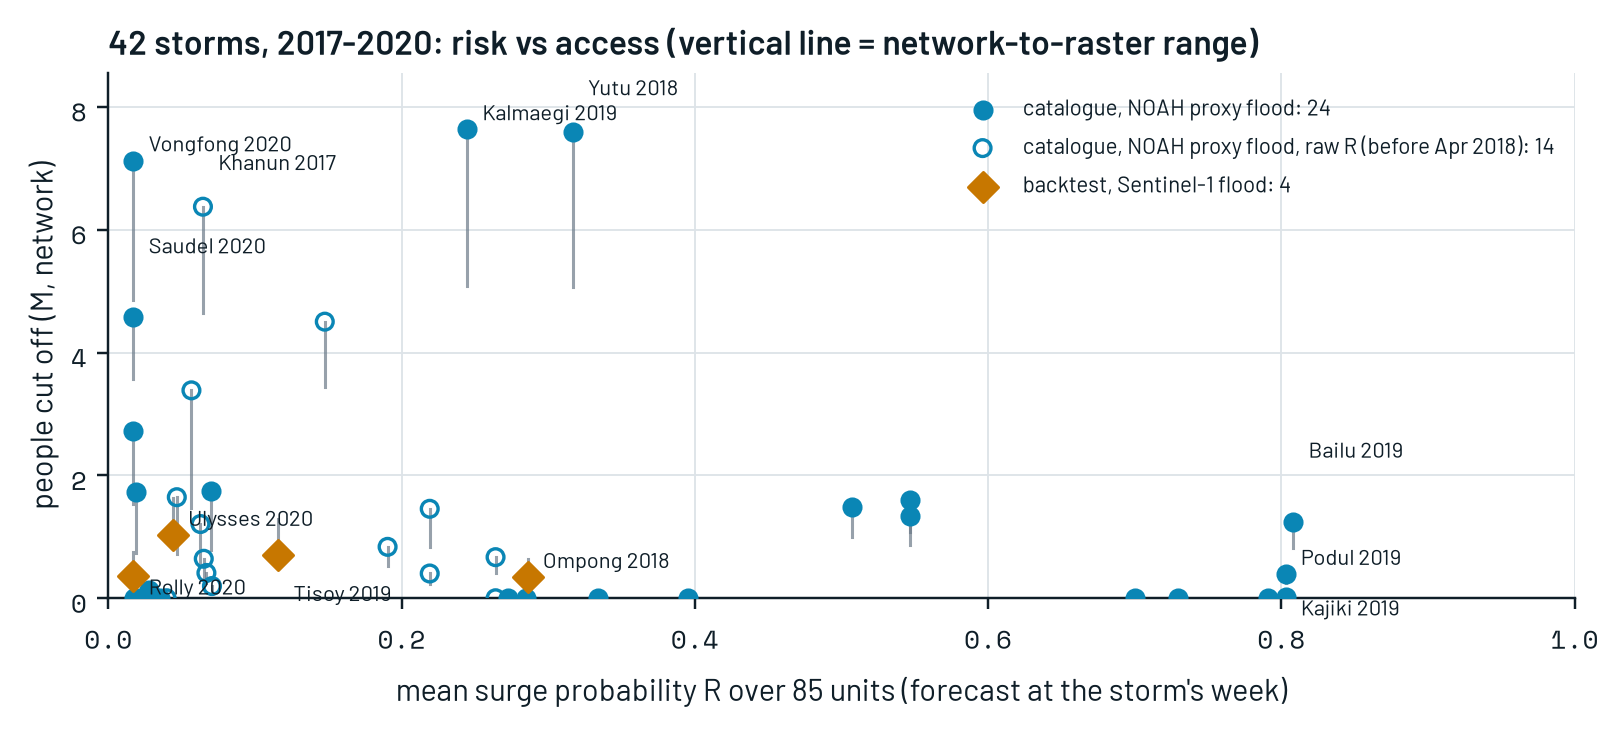
\includegraphics[width=\linewidth]{f16_catalog}
\caption{Mean surge probability and people cut off per storm. Diamonds: the four backtests (Sentinel-1 flood, lower bounds); circles: catalogue storms (NOAH proxy, upper bounds); hollow: raw $R$. The vertical line spans the network-to-raster range.}
\label{fig:catalog}
\end{figure}

\begin{table}[htbp]
\centering
\caption{Every scored storm in date order. $R$: mean over the \nUnits{} units; cut: people cut off (millions), network and raster; $R \times$cut: expected people at surge risk who are cut off ($\Sigma\, R \times$ cut off over units); D/P: provinces at deploy / pre-position. $\blacklozenge$ backtest (Sentinel-1); \textsuperscript{\dag} raw $R$ (before calibration was possible).}
\label{tab:catalog}
\scriptsize
\begin{tabular}[t]{@{}l r r r r r r@{}}
\toprule
storm & $R$ & cut & raster & $R \times$cut & ferry & D/P \\
\midrule
\tablerows{catalogA}
\bottomrule
\end{tabular}\hfill
\begin{tabular}[t]{@{}l r r r r r r@{}}
\toprule
storm & $R$ & cut & raster & $R \times$cut & ferry & D/P \\
\midrule
\tablerows{catalogB}
\bottomrule
\end{tabular}
\end{table}

The largest cut-offs (\largestCutStorms{}) pair with low $R$; the high-$R$ storms (\highRStorms{}) came in the 2019 epidemic season. The network and raster agree across units with a median $\rho$ of \catRhoMedian{} (minimum \catRhoMin{}) over the \catRhoN{} storms with any cut-off.
